% !TeX encoding = UTF-8 Unicode 
%Tiedoston merkistö

\documentclass[finnish]{article}


\usepackage{array}
\usepackage{pgf}
\usepackage{tikz}
\usetikzlibrary{arrows,automata}

\usepackage{babel,t1enc} %,times} % Suomen tavutus

\usepackage[utf8]{inputenc} % näppäimiltä tuleva merkistö
\usepackage{geometry}
\geometry{margin=2.54cm,a4paper}  % paperin koko
%\geometry{margin=2.54cm}

\usepackage{lastpage}
\usepackage{fancyhdr}
\pagestyle{fancy}
\fancyhf{} % clear all header and footer fields
\renewcommand{\headrulewidth}{0pt}
\cfoot{\thepage\ (\pageref{LastPage})}


\usepackage{amssymb,amsmath,mycode}
%\input{../macs/macs}
%\input{bwmacs}


\usepackage{graphicx}

\usepackage{multirow}


\newcommand{\set}[1]{{\left\{ #1 \right\}}}

\begin{document}

\subsection*{582206 Laskennan mallit (syksy 2012)\\
{\rm Harjoitus 3 (17.--20.9.)}}

\bigskip 

\begin{enumerate}


\item 
\begin{tabular}[t]{p{6cm}c}
\multirow{2}{7cm}{%
Olkoon $N_1$ ja $N_2$ epädeterministiset automaatit jotka on kuvattu oikealla.
Tunnistavatko automaatit seuraavat sanat? 
\begin{enumerate}
\item $a$
\item $aa$
\item $aab$
\item $\varepsilon$
\item $ab$
\item $abab$
\item $aba$
\item $abaa$
\end{enumerate}
} 

&

\begin{tabular}{cm{4cm}}
$N_1:$ &
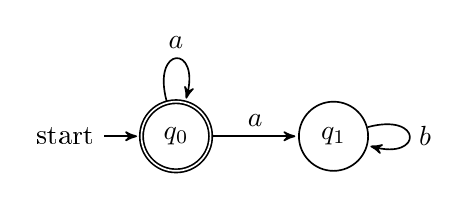
\begin{tikzpicture}[->,>=stealth',shorten >=1pt,auto,node distance=2cm,semithick]
 %\tikzstyle{every state}=[fill=red,draw=none,text=white]

 \node[state,initial,accepting] (q0)               {$q_0$};
 \node[state]                   (q1) [right of=q0] {$q_1$};

 \path (q0) edge [loop above]  node      {$a$}   ()
            edge               node     {$a$}  (q1)
       (q1) edge  [loop right]       node       {$b$}  ();
\end{tikzpicture} 
\end{tabular}

\\[2cm]

 & 
\begin{tabular}{cm{4cm}}
$N_2:$ &
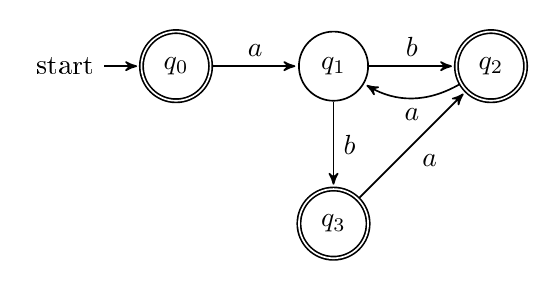
\begin{tikzpicture}[->,>=stealth',shorten >=1pt,auto,node distance=2cm,semithick]
 %\tikzstyle{every state}=[fill=red,draw=none,text=white]

 \node[state,initial,accepting]	(q0)               {$q_0$};
 \node[state]   				(q1) [right of=q0] {$q_1$};
 \node[state,accepting]         (q2) [right of=q1] {$q_2$};
 \node[state,accepting]         (q3) [below of=q1] {$q_3$};
 
 \path (q0) edge   				node		{$a$}  	(q1)
       (q1) edge   				node 		{$b$}  	(q2)
            edge   				node 		{$b$} 	(q3)
       (q2)	edge [bend left]	node    	{$a$}	(q1)       
       (q3) edge				node [swap]	{$a$}	(q2);        
\end{tikzpicture}
\end{tabular}
\end{tabular}



\item Minkälaisia sanoja seuraavat äärelliset epädeterministiset automaatit hyväksyvät?

\begin{enumerate}
\item 
\begin{tabular}{c}
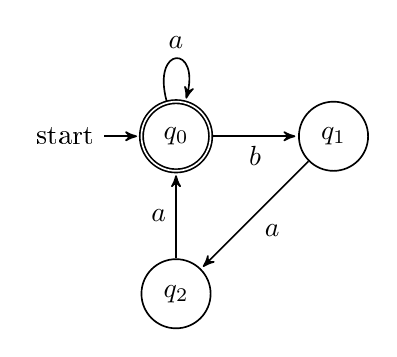
\begin{tikzpicture}[->,>=stealth',shorten >=1pt,auto,node distance=2cm,semithick]
 %\tikzstyle{every state}=[fill=red,draw=none,text=white]

 \node[state,initial,accepting] (q0)               {$q_0$};
 \node[state]                   (q1) [right of=q0] {$q_1$};
 \node[state] (q2) [below of=q0] {$q_2$};

 \path (q0) edge [loop above]  node      {$a$}   ()
            edge               node [swap]{$b$}  (q1)
       (q1) edge               node       {$a$}  (q2)
       (q2) edge               node       {$a$} (q0);
\end{tikzpicture}
\end{tabular}

\item 
\begin{tabular}{c}
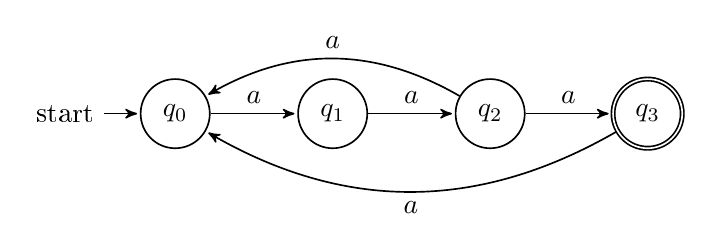
\begin{tikzpicture}[->,>=stealth',shorten >=1pt,auto,node distance=2cm,semithick]
 %\tikzstyle{every state}=[fill=red,draw=none,text=white]

 \node[state,initial]   (q0)               {$q_0$};
 \node[state]           (q1) [right of=q0] {$q_1$};
 \node[state]           (q2) [right of=q1] {$q_2$};
 \node[state,accepting] (q3) [right of=q2] {$q_3$};

 \path (q0) edge               node      {$a$}   (q1)
       (q1) edge               node       {$a$}  (q2)
       (q2) edge               node       {$a$} (q3)
            edge  [bend right] node [swap]{$a$} (q0)
       (q3) edge  [bend left]  node       {$a$} (q0);
\end{tikzpicture}
\end{tabular}
\end{enumerate}



\item Piirrä epädeterministiset automaatit tiloineen ja siirtymänuolineen seuraaville kielille.
\begin{enumerate}
\item $L = \set{w \in \set{a, b}^* \mid \mbox{$w$ sisältää korkeintaan kaksi $a$:ta}}$
\item $L = \set{w \in \set{a, b}^* \mid \mbox{$w$ sisältää parillisen määrän alimerkkijonoa $ab$}}$
\item $L = \set{w \in \set{a,b}^*  \mid \mbox{$w$:n ensimmäinen ja viimeinen kirjain ovat samat}}$
\end{enumerate}



\item
Merkkinon $w=w_1 w_2 \dots w_n$ \textit{käänteismerkkijono} on $w^{{\cal R}}=w_n w_{n-1}\dots w_1$.  Olkoon kielen $A$ \textit{käänteiskieli} $A^{{\cal R}} = \set{w^{{\cal R}}\mid w \in A}$. Näytä että jos $A$ on säännöllinen niin myös $A^{{\cal R}}$ on säännöllinen (vihje: käytä epädeterministisyyttä apuna). Tee myös pienet esimerkit.


\item
Muunna seuraavat epädeterministiset automaatit deterministisiksi käyttämällä lauseen 1.39 todistusta apuna.

\begin{tabular}{cc}
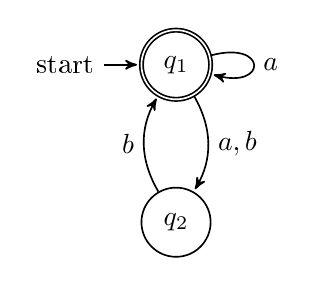
\begin{tikzpicture}[->,>=stealth',shorten >=1pt,auto,node distance=2cm,semithick]

 \node[state,initial,accepting] (q1)               {$q_1$};
 \node[state]                   (q2) [below of=q1] {$q_2$};

 \path (q1) edge [loop right]  node      {$a$}   ()
            edge  [bend left]       node     {$a,b$}  (q2)
       (q2) edge  [bend left]       node       {$b$}  (q1);
\end{tikzpicture} 
 & 
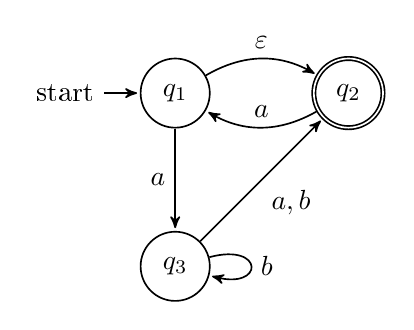
\begin{tikzpicture}[->,>=stealth',shorten >=1pt,auto,node distance=2.2cm,semithick]

 \node[state,initial]	(q1)  				{$q_1$};
 \node[state,accepting]	(q2) [right of=q1] {$q_2$};
 \node[state]   		(q3) [below of=q1] {$q_3$};
 
 \path (q1) edge   				node [swap]	{$a$}  	(q3)
            edge [bend left] 	node 		{$\varepsilon$} 	(q2)
       (q2)	edge [bend left]	node [swap]   	{$a$}	(q1)       
       (q3) edge				node [swap]	{$a,b$}	(q2)
            edge [loop right]   node    {$b$} ();        
\end{tikzpicture}
\end{tabular}


\item 
Olkoon $M$ \textbf{deterministinen} automaatti, missä on $n$ tilaan, ja $L(M)=A$. (vihje ajattele syklejä)
\begin{enumerate}
\item Todista että $A\neq \emptyset$ jos ja vain jos $\exists w \in A$ mille $|w| < n$.
\item
Todista että $A$ on ääretön jos ja vain jos $\exists w \in A$ mille $n \le |w| < 2n$
\end{enumerate}




%\item 
%Olkoon 
%\[ \Sigma_3 = \set{
%\begin{bmatrix} 0 \\ 0 \\ 0 \end{bmatrix},
%\begin{bmatrix} 0 \\ 0 \\ 1 \end{bmatrix}, \dots ,
%\begin{bmatrix} 1 \\ 1 \\ 1 \end{bmatrix}
%}\,.
%\]
%$\Sigma_3$ koostuu siis kolmen kokoisista sarakeista, jotka sisältävät nolli ja ykkösiä.
% taulukoista. Olkoon 
%\[
%B=\set{w \in \Sigma_3^* \mid \mbox{w:n alimmainenn numero on ylimmäisten summa}}\,.
%\]
%Esimerkiksi
%\[ 
%\begin{bmatrix} 0 \\ 0 \\ 1 \end{bmatrix}
%\begin{bmatrix} 1 \\ 0 \\ 1 \end{bmatrix}, \dots ,
%\begin{bmatrix} 1 \\ 1 \\ 1 \end{bmatrix}
%\]
%



\end{enumerate}


\end{document}
